%!TEX root = ../../master.tex
\section{Our Definition}
A clarification of what is meant by resilience in distributed systems is needed since the term is getting more attention. In this section, we will define a subset of resilience in the context of distributed systems and cloud computing from our perspective and experiences.

\begin{figure}[H]
    \centering
    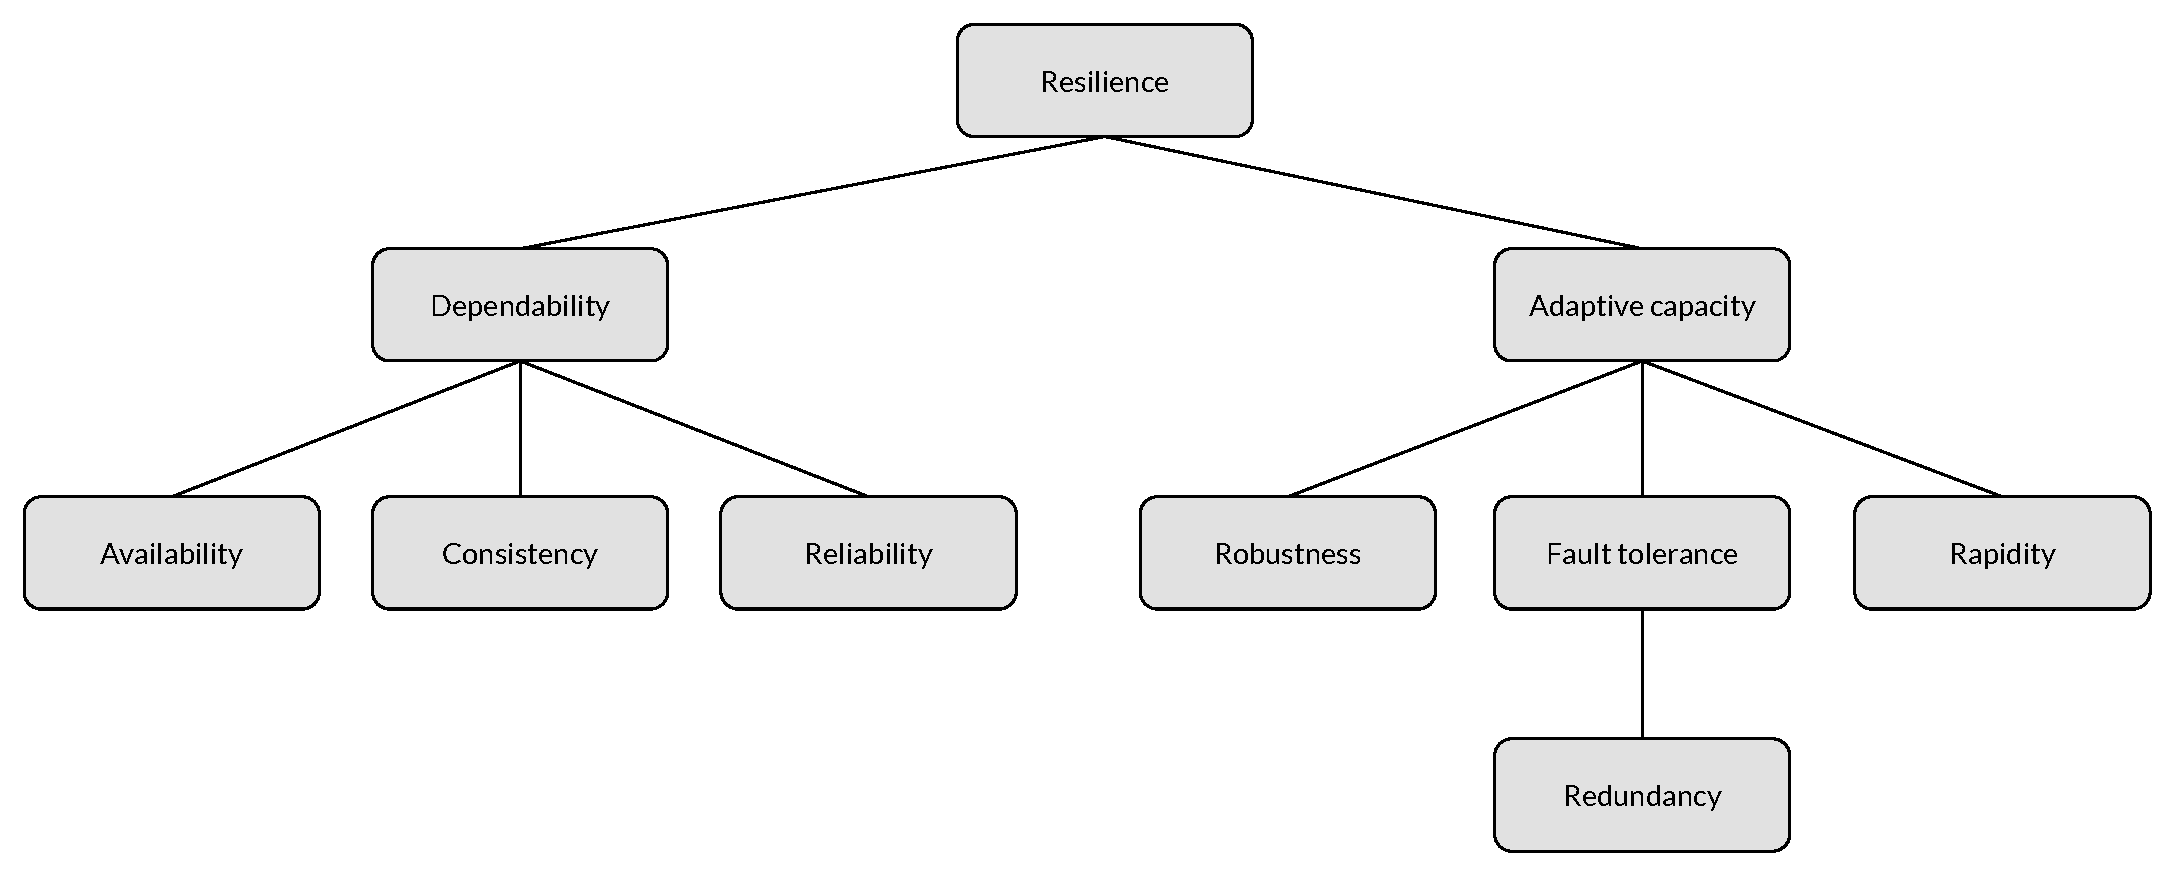
\includegraphics[width=\textwidth]{figures/our_resilience}
    \caption{Our Resilience Definition}
    \label{fig:our_resilience_definition}
\end{figure}

\noindent The illustration of resilience (Figure~\ref{fig:our_resilience_definition}) shows characteristics of resilience with interconnected concepts. Dependability has been described for software for many years. An attribute such as \textit{availability} has been described as the \textit{"readiness of a service"}. Similarly \textit{reliability} has been described as the \textit{"continuity of a correct service"} \cite[p. 2]{Laprie1995}. We argue that there is a lack of focus on the granularity of consistency. Ensuring high availability is often traded off by prioritizing consistency lower. Section~\ref{sec:exp_integration_points} investigates to what extent this trade-off can be done, and quantifies the effect. The experiment is conducted by introducing errors while measuring how a circuit breaker, explained later, can help. \\

\noindent
The adaptive capacity, the right-hand side (Figure~
\ref{fig:our_resilience_definition}), is another important factor for resilience, which is similar to resourcefulness. Being able to adapt is important in an ever-changing environment, which leads to the following desired characteristics. Robustness refers to standing against stress or potential disruptions and avoid failure. Fault tolerance refers to continuing when faults or errors happen, and a mean to this is redundancy. The last concept is rapidity which refers to mitigating the impact of failure and recovering to normal service. Section~\ref{sec:exp_replication} investigates these concepts by quantifying how an infrastructure, in this case Kubernetes, can detect, mitigate, and handle faults, when a service becomes unavailable due to a network error. Furthermore, the effect of running multiple replicas for robustness is investigated and quantified.

